%\documentclass[aps,prl,twocolumn,nobibnotes]{revtex4}
\documentclass[aps,showpacs,twocolumn,nobibnotes]{revtex4}
%\documentclass[aps,preprint,showpacs,nobibnotes]{revtex4}
%\documentclass[aps,preprint,nobibnotes]{revtex}
\usepackage{graphics,graphicx,amsfonts,amsmath,amsbsy,amssymb,color}
\usepackage{bm}
%\usepackage{epic}
%\usepackage{mciteplus}
\usepackage{subfigure}
\usepackage{vector}  % Allows "\bvec{}" and "\buvec{}" for "blackboard" style bold vectors in maths
\newcommand{\D}[1] {D_{\bf #1}}
\def \beq {\begin{eqnarray}}
\def \eeq {\end{eqnarray}}
\def \Schrodinger {{Schr\"{o}dinger }}
\def \Di {{D_{\bfi}}}
\def \Dj {{D_{\bfj}}}
\newcommand {\adag}[1] {{a_{#1}^\dagger}}
\def \bfj {{\bf j}}
\def \bfi {{\bf i}}
\def \rone {{\bvec{r}_1}}
\def \rtwo {{\bvec{r}_2}}
\def \mEh {{\textrm{mE}_{\textrm{h}}}}
\def \Eh {{\textrm{E}_{\textrm{h}}}}
\def \nadd {{n_a}}
\newcommand{\braket}[3] {{\langle #1 | #2 | #3 \rangle}}
\newcommand{\brket}[2] {{\langle #1 | #2 \rangle}}
\newcommand{\bra}{\ensuremath{\langle}}
\newcommand{\ket}{\ensuremath{\rangle}}
%\def \ham {{\bf H}}
\def \ham {{\hat{H}}}
%\def \Sz {{\hat{\textrm{S}_{\textrm{z}}}}}
\def \Sz {{\hat{S}_z}}
\newcommand{\rff}[1]{{Eq.~\eqref{#1}}}
\def \Pgen {{P_{\textrm{gen}}}}
\def \Carb {{\textrm{C}_{\textrm{2}}}}
\def \Hij {{H_{\bvec{i}\bvec{j}}}}
\def \Kii {{K_{\bvec{i}\bvec{i}}}}
\def \Kij {{K_{\bvec{i}\bvec{j}}}}

\begin{document}
\title{Spectral functions of extended systems via quantum embedding}
\author{George~H.~Booth}
%\email{ghb24@cam.ac.uk}
\author{Garnet~Kin-Lic~Chan}  
\affiliation{Department of Chemistry, Frick Laboratory, Princeton University, Princeton, New Jersey 08544, USA}

\begin{abstract}
In a previous publication [PRL {\bf 109} 186404 (2012)], the ground-state density matrix embedding theory (DMET) was introduced. With similarities 
to the dynamical mean-field method, a set of local sites are self-consistently correlated, but with an analytically constructable bath describing the
coupling to the rest of the extended system. 
Despite many formal advantages in the analytic embedding, the method was restricted to static, ground-state properties.
Here, we extend the approach to introduce a frequency dependence, and demonstrate accurate spectral functions at a small 
computational cost. In a similar spirit to the frequency independent DMET method, the impurities are coupled via a small set of 
analytically constructed, but now frequency-dependent bath states. In contrast to dynamical mean-field theory, the resultant 
spectral functions are directly obtained on the real-frequency axis, with no bath discretization error and allow for straightforward generalization both 
to impurity clusters and arbitrary electron perturbation operators. We demonstrate
the application of this method on the hubbard model, where both the the Kondo resonances and metal-insulator transitions are well reproduced, as well as 
demonstrating two-electron spectra. This vastly extends the scope and applicability 
of the DMET method in condensed matter problems as a cheap route to correlated local spectral functions of extended systems.
\end{abstract}
\date{\today}
\maketitle

Dynamic correlation functions are directly probed in spectroscopic methods, and correspond to many of the important transport, optical and 
wider electronic structure properties of materials. As such, their accurate theoretical construction is key for materials scientists. 
However, few robust approaches exist for strongly correlated problems. The difficulty is in simultaneously requiring both an accurate 
treatment of the electron correlations beyond mean-field band theory for 
ground states, as well as the excitation spectrum coupled to the infinite bulk
system.

all excited state components at each frequency, as well as 
convergence with respect to the finite-size effects in the solid state. In dynamical mean-field theory (DMFT), the central quantity 
is the greens function of the system, which is self-consistenty optimized 

Difficulty with optical spectra - 
Not constrained by finite size effects which have plagues QMC and ED calculations.

Regularized by addition of small imaginary component to the energy for spectral broadening.

Disadvantages of DMFT:

Size of bath independent of the size of the underlying lattice. Only a function of the impurity cluster size and the perturbation, while still exact in the non-interacting limits.
Althugh the single-particle density of states is crucial STM/ARPES, other spectral functions are also highly sought after in materials science, such as the 
Two-hole propagator, probed with Auger spectroscopy (PRB 87, 165136 (2013), the two-electron neutral excitation spectrum, a key quantity in the mechanism of high-temperature superconductivity and Raman spectroscopy (Millis), as well as other important correlation functions such as the dynamic polarizability.

Coupling only within the bandwidth of the 1 electron bath
Plotted within the bandwidth of the 1 electron 

1 electron response operator is partitioned into the schmidt basis, such that a block acts purely in the schmidt basis of the ground state embedded space, 

Schmidt decompose the action of the non-interacting operator, into that acting on the space of the impurity+bath ground state system, and that acting on the rest of the environment orbitals.

Cost of any frequency point not more than a minute on a single processor core.

DD results using reoptimized ground state.

Within the 1 electron response function bandwidth

Doped Spectral functions in 1D with DMRG: PRL (2004) 256401, 92

ED can only treat small clusters, and therefore the relatively small numbers of poles that are unable to be resolved into the spectral functions of the extended system. Perturbation theory, 
correlation only treated to low order, and will 
lose accuracy as you tend towards to opposite coupling limit to the zeroth order solution (PRL 84 522 1999), and QMC is formulated in imaginary time, and therefore the maximum entropy is needed,
washes out the subtle feature of the spectrum.


Gap measured from Single-particle spectrum as the difference between the energy of the lowest electron peak and that of the highest hole peak in the single-particle DoS.

Continuous Weiss field approximated by a finite number of bath sites - require convergence with respect to this parameter, while computational effort will generally increase exponenetially wrt this number.

Can be computed via the 1-particle or 2-particle greens function

Possible to reoptimize the ground state in the space of V*|0>, but this was found not to materially change results, and so is not performed from the results presented here.

%+++++++++++++++++++++++++++++++++++++++++++++++++++++++
%   1D HUBBARD MODEL PLOTS vs. CDMFT
%+++++++++++++++++++++++++++++++++++++++++++++++++++++++
\begin{figure}
\begin{center}
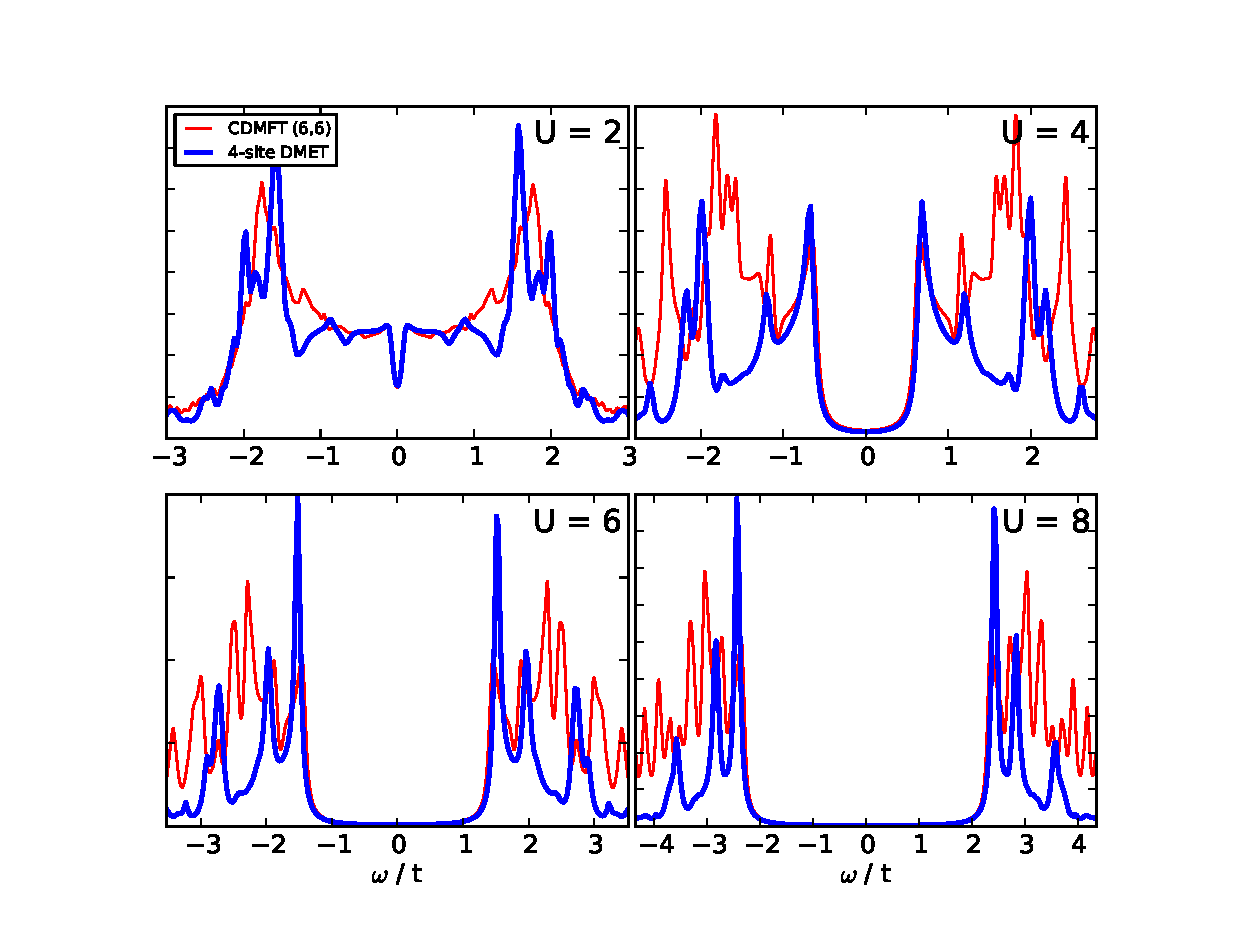
\includegraphics[scale=0.475]{Plots/1D_Spectra/1D_Hub_Spectra.eps}
\end{center}
\caption{Comparison of the local density of states from a four impurity cluster DMET calculation with a
(six impurity, six bath) CDMFT calculation for the half-filled 1D Hubbard model.}
\label{1D_DOS}
\end{figure}

%+++++++++++++++++++++++++++++++++++++++++++++++++++++++
%   1D HUBBARD SPECTRAL GAP 
%+++++++++++++++++++++++++++++++++++++++++++++++++++++++
\begin{figure}
\begin{center}
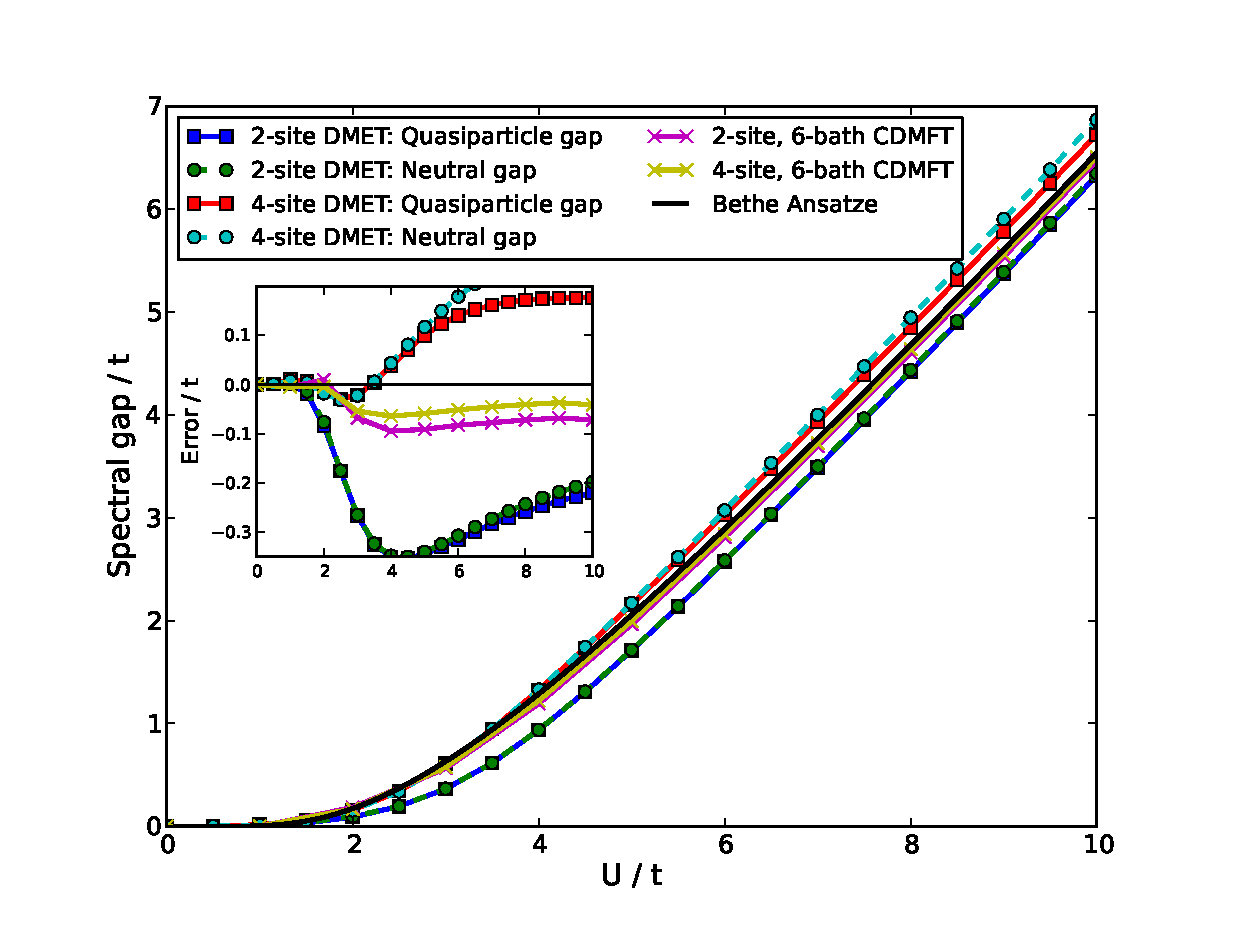
\includegraphics[scale=0.475]{Plots/1D_Gap/Hubbard_Gap.eps}
\end{center}
\caption{Spectral gap from the 1-particle and 2-particle greens functions compared to analytic results
from the Bethe Ansatze\cite{Ovchinni1970}.}
\label{1D_GAP}
\end{figure}


%+++++++++++++++++++++++++++++++++++++++++++++++++++++++
%   2D HUBBARD PLOTS 
%+++++++++++++++++++++++++++++++++++++++++++++++++++++++
\begin{figure}
\begin{center}
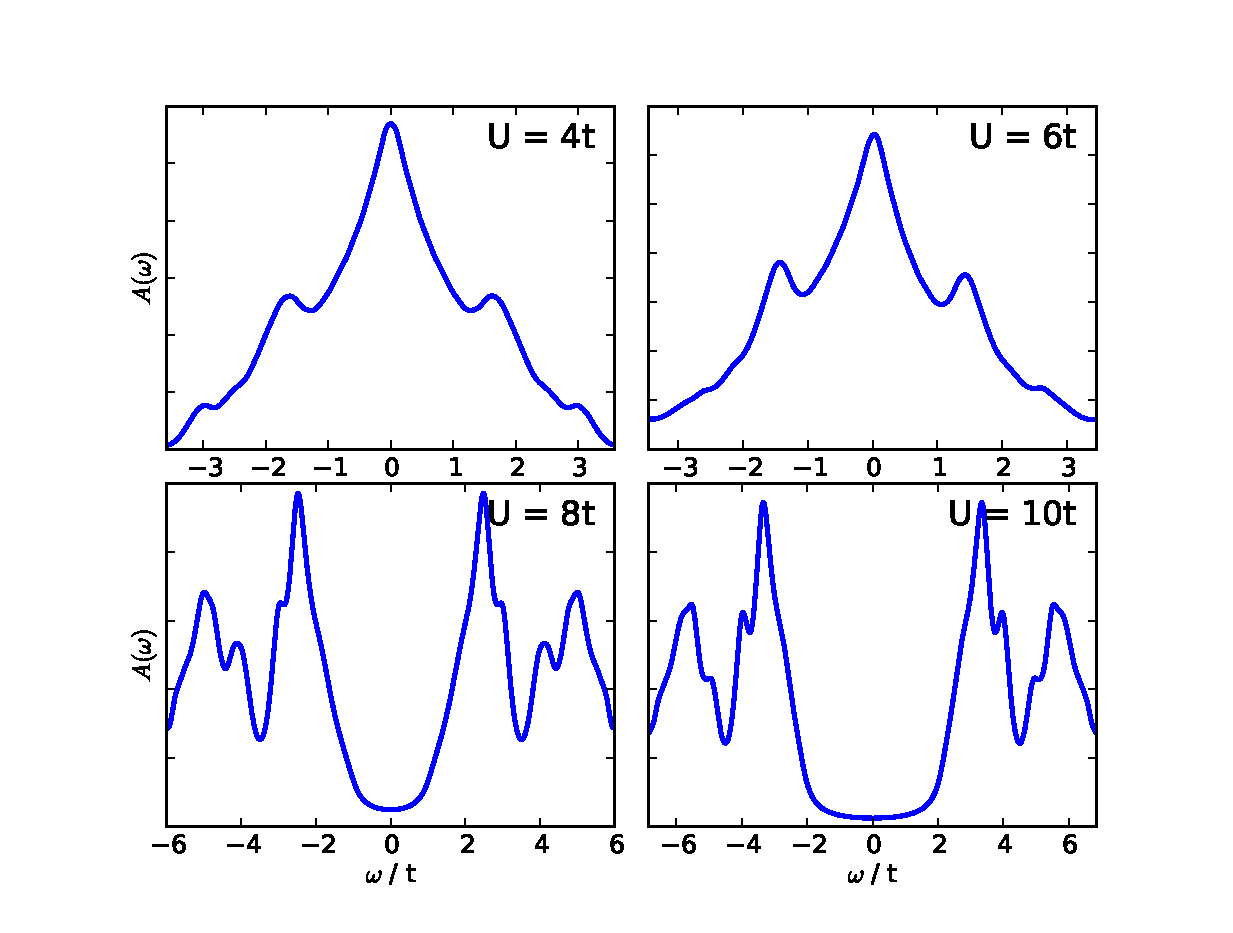
\includegraphics[scale=0.475]{Plots/2D_Spectra/2DHub_Spectra.eps}
\end{center}
\caption{Local density of states of the half-filled 2D hubbard model from a four impurity DMET calculation.}
\label{2D_DOS}
\end{figure}


%+++++++++++++++++++++++++++++++++++++++++++++++++++++++
%   2D DOPED HUBBARD PLOTS 
%+++++++++++++++++++++++++++++++++++++++++++++++++++++++
\begin{figure}
\begin{center}
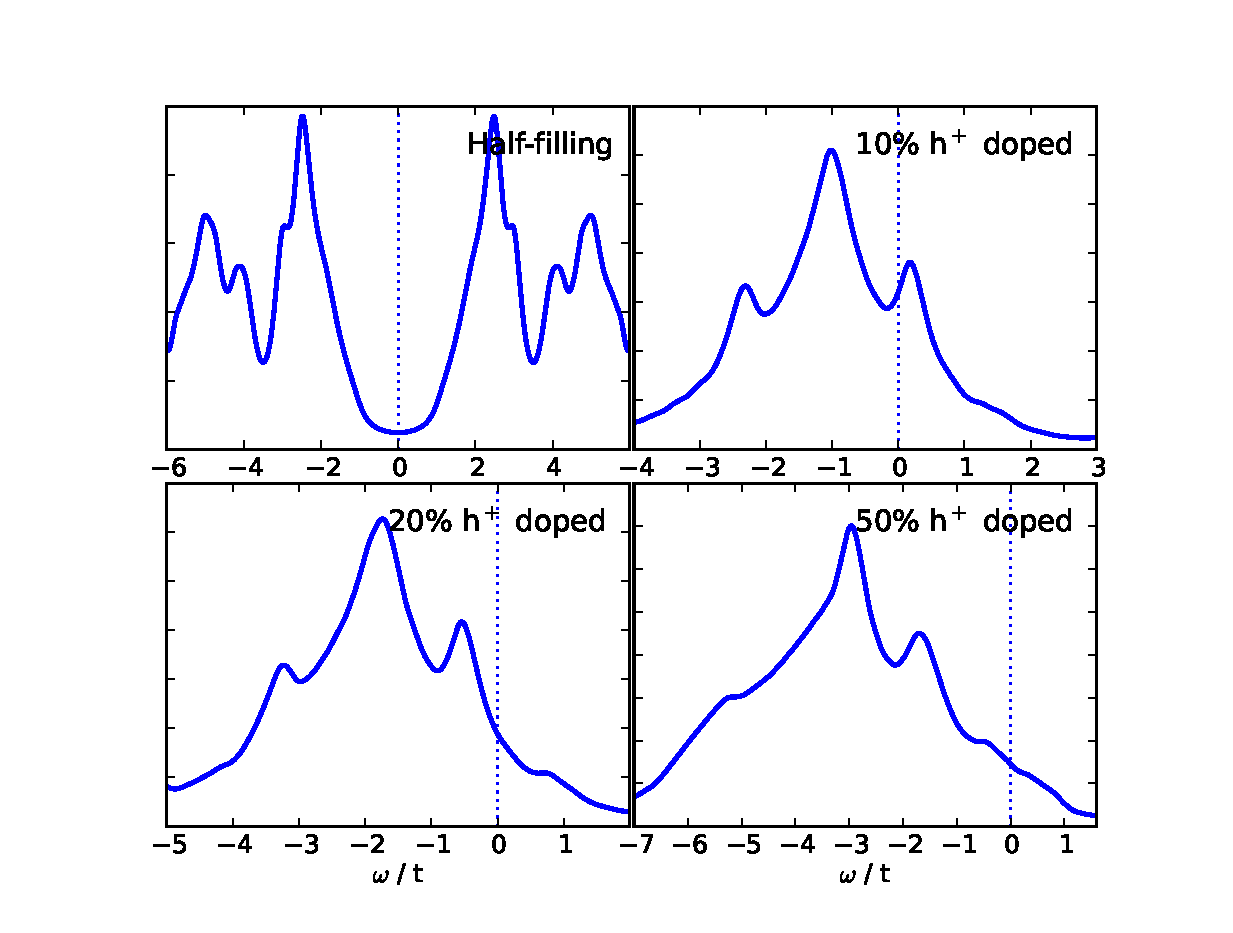
\includegraphics[scale=0.475]{Plots/Doping/2D/nImp4/U8/LargerBroadening/2DHub_Doping.eps}
\end{center}
\caption{Local density of states of the hole doped 2D hubbard model from a four impurity DMET calculation with $U = 8t$.}
\label{2D_Doped}
\end{figure}

%+++++++++++++++++++++++++++++++++++++++++++++++++++++++
%   DD response 
%+++++++++++++++++++++++++++++++++++++++++++++++++++++++
\begin{figure}
\begin{center}
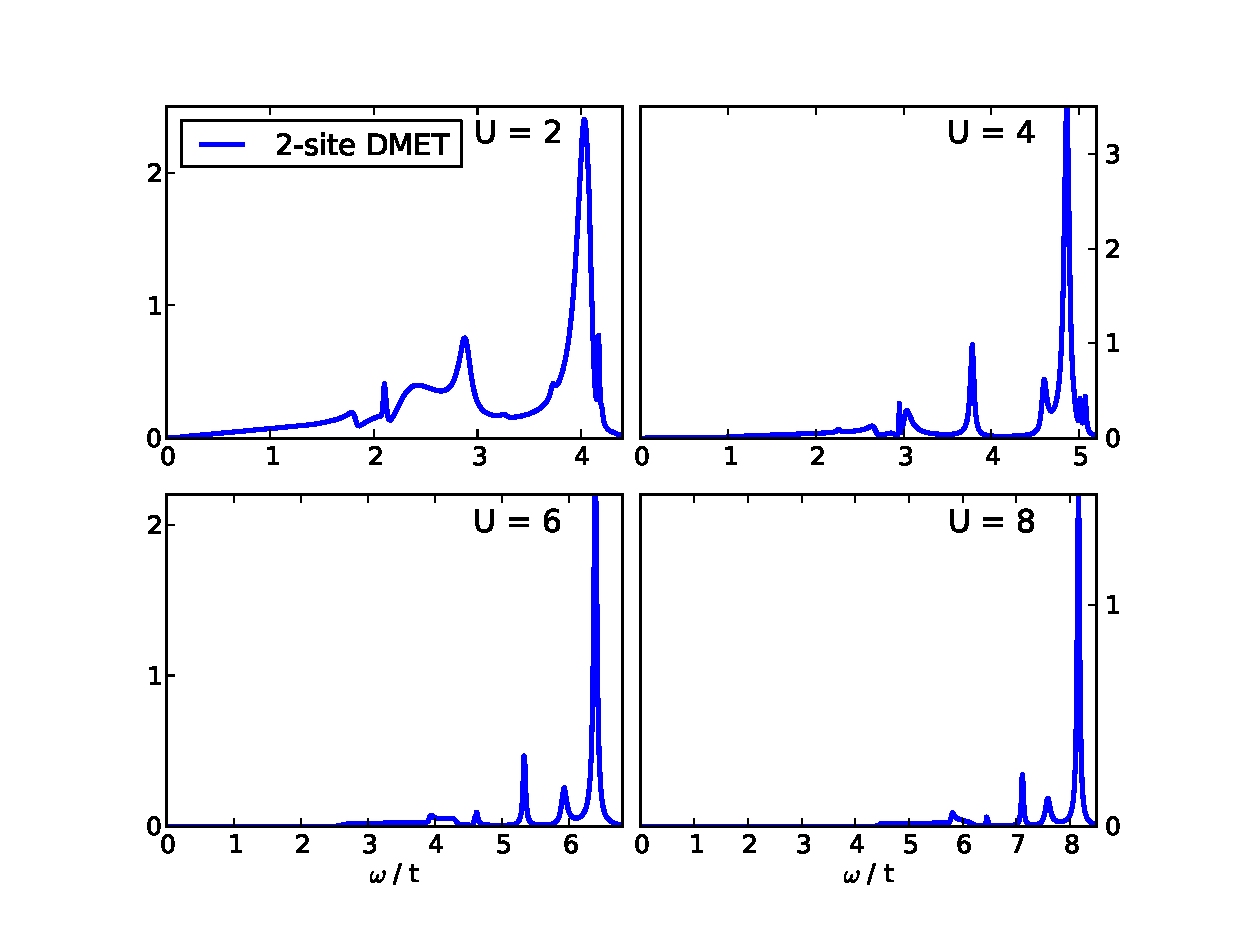
\includegraphics[scale=0.475]{Plots/1D_DD/1D_Hub_DD.eps}
\end{center}
\caption{Two impurity DMET calculation of the local density-density response function for the half-filled 1D hubbard model via construction of the 2-particle greens function.
The spectral gap is used in the data plotted in Fig.~\ref{1D_GAP}}
\label{1D_DD}
\end{figure}



\bibliography{SpectralDMETBib}

\end{document}
